\documentclass[a4paper]{article}
\usepackage[utf8]{inputenc}
\usepackage[T1]{fontenc}
\usepackage{times}
\usepackage[margin=3cm]{geometry}
\usepackage{float}

% German
%\usepackage[ngerman]{babel}
% English
\usepackage[english]{babel}

\usepackage[round,authoryear]{natbib}
\usepackage{amsmath,amssymb,amsthm}
\usepackage[hyphens]{url}
\usepackage{graphicx}
\usepackage{booktabs}

\usepackage{lipsum}

% German
%\newtheorem{definition}{Definition}
%\newtheorem{satz}{Satz}
% English
\newtheorem{definition}{Definition}
\newtheorem{theorem}{Theorem}

% TODO
\author{A. Student}
\title{Performance and Privacy Mechanisms in CODoH: Cacheable Oblivious DNS over HTTPS}
\date{\today}

\begin{document}

\maketitle

\begin{abstract}
  Oblivious DNS over HTTPS (ODoH) improves DNS privacy by separating users' identities from their queries. However, this prevents intermediary proxies from caching responses, increasing DNS resolution latency. Cacheable Oblivious DNS over HTTPS (CODoH) addresses this limitation by introducing privacy-preserving caching. In this report, we examine CODoH's design and the security mechanisms used to prevent attackers from inferring sensitive information through cache behavior. We also analyze the performance results reported by its authors, which show substantial latency reductions for repeated queries while maintaining similar performance for uncached queries. These improvements come at the cost of additional network traffic and processing overhead.
\end{abstract}

\section{Introduction}
\label{sec:intro}
The Domain Name System (DNS) is a fundamental component of the Internet, responsible for translating human-readable domain names into IP addresses \citep{rfc1034}. Most interactions with the internet require DNS resolution, which makes DNS queries a source of information for users' online activity. Originally, DNS queries have been transmitted without encryption, allowing all intermediaries with access to the packet to observe which domains users access \citep{rfc9076}. Protocols such as DNS over HTTPS (DoH), DNS over TLS (DoT) and DNS over QUIC (DoQ) have been invented to provide a solution for this issue by encrypting the communication between clients and DNS servers \citep{rfc8484,rfc7858,rfc9250}. However, while these protocols protect DNS queries from intermediaries in the network, the DNS server can still associate a query to the IP Address of the user that issued them.

Oblivious DNS over HTTPS (ODoH) addresses this issue by introducing an intermediary proxy that separates the client's identity from the query contents, forwarding encrypted requests to the target DNS server, which ensures that neither the proxy or the DNS server possess both the user's identity and the query contents \citep{singanamalla2020oblivious,rfc9230}. Although this approach guarantees the privacy of the client's request end to end, it also prevents intermediary proxies from caching requests, since the query contents only get decrypted at the target resolver.

To overcome this issue, \citet{niroula2026codoh} developed Cacheable Oblivious DNS over HTTPS (CODoH) protocol. Rather than simply decrypting and caching DNS queries, CODoH combines trusted execution environments with techniques to prevent cache access patterns from revealing information. Its objective is to preserve the privacy properties of ODoH while partly recovering the performance benefits of DNS caching. However, these mechanisms also introduce overhead, raising questions about the performance of CODoH.

This report examines and discusses the privacy-enhanced mechanisms suggested by CODoH as well as its effects on performance.



\section{Background}
\label{sec:background}

\subsection{DNS \& DNS Caching}
\label{sec:dnsanddnscaching}

The \textit{Domain Name System (DNS)} is a distributed naming system that allows mapping domain names into certain information, usually into IP addresses \citep{rfc1034}. When a client needs to resolve a domain address, usually it sends a query to a recursive \textit{DNS resolver}, which may contact multiple DNS servers following the DNS hierarchy, as illustrated in Figure~\ref{fig-resolution-process}. For example, a client may request the DNS resolver the resolution of the domain "example.com". In such case, the DNS resolver will initially query the Root Server to get the Top Level Domain (TLD) server information. Then, it will query the TLD server ".com" to obtain the authoritative Name Server (NS) of "example.com". Finally, it will query the NS to obtain the corresponding IP Address, and answer the original client.

\begin{figure}[H]
	\centering
	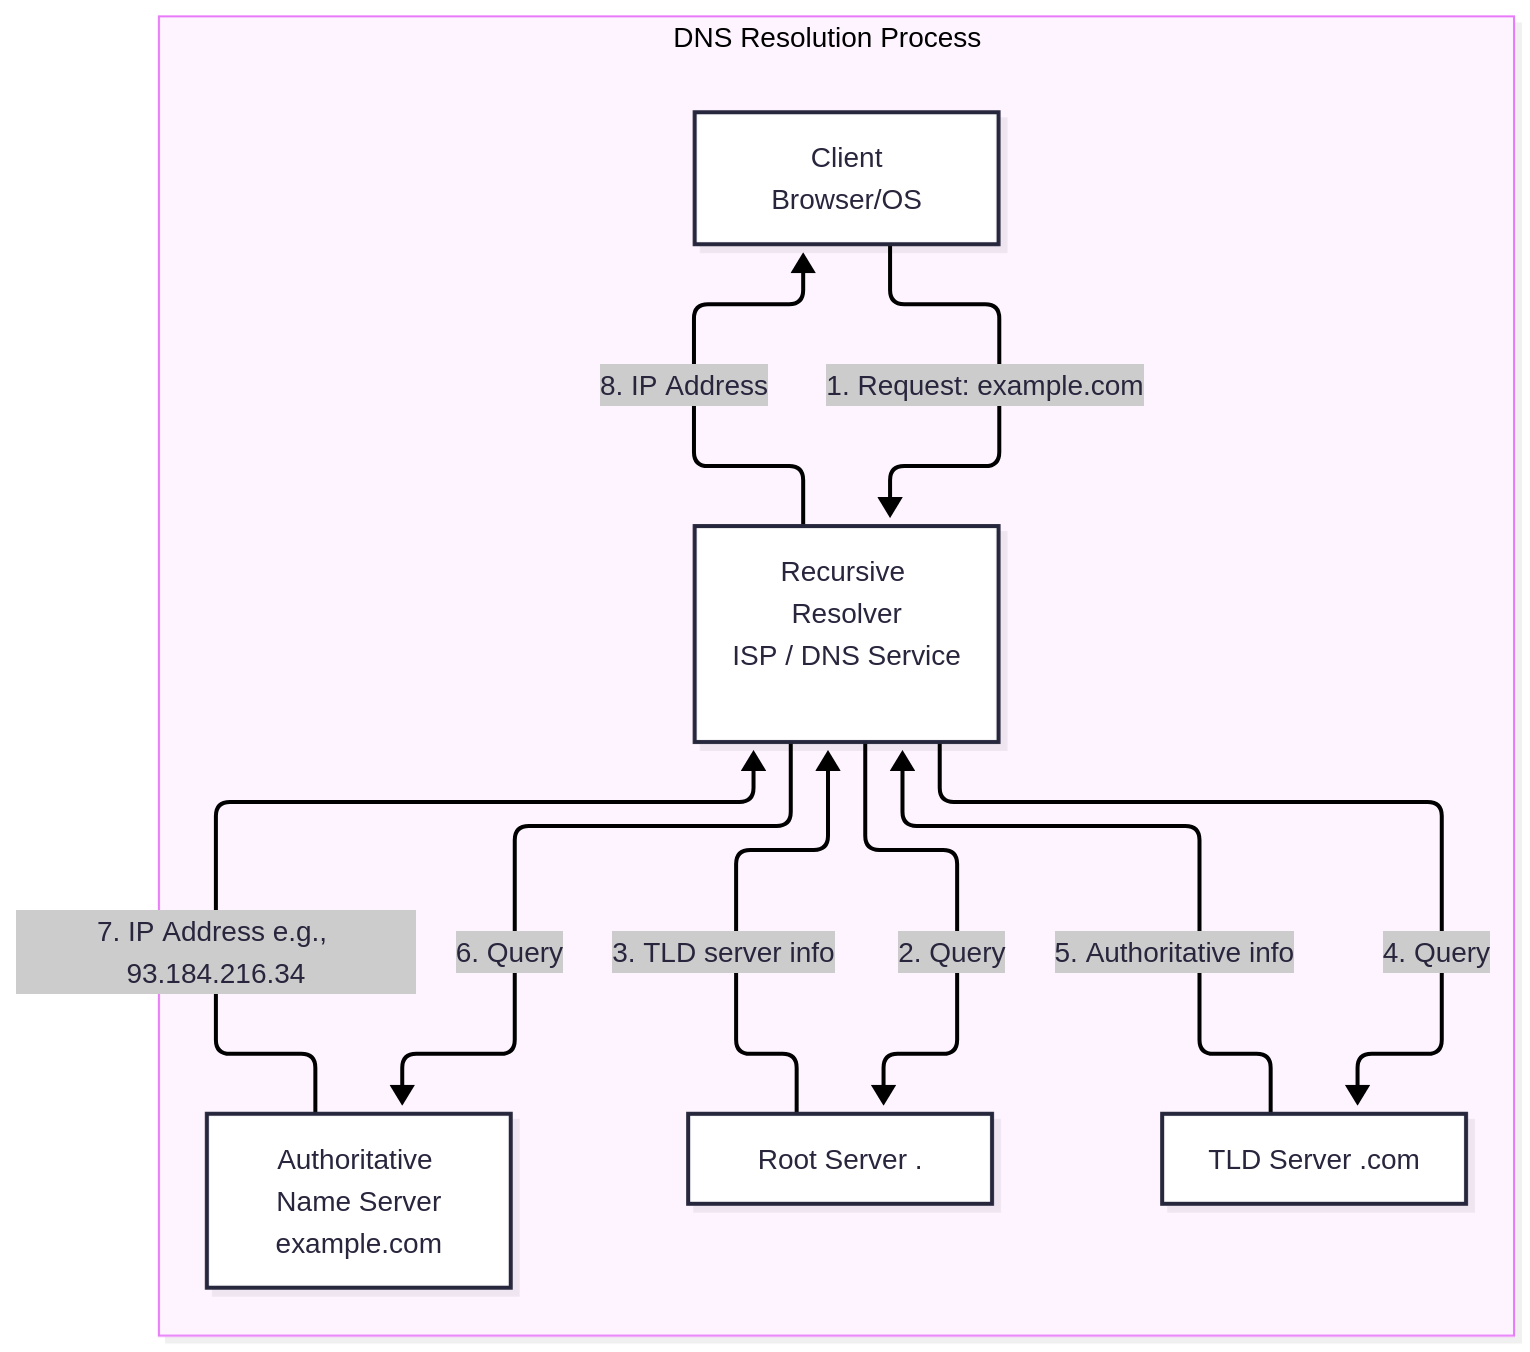
\includegraphics[width= 0.6\textwidth]{figures/dns-resolution-process}
	\caption[DNS resolution process]{
		DNS resolution process.
		Initially generated using Gemini 4 Argon with the prompt
		``Generate a high-level mermaid diagram illustrating DNS resolution
		with a recursive resolver'' on 17.10.2026, modified by the author.
		
	}
	\label{fig-resolution-process}
\end{figure}

To reduce the overhead associated with the DNS resolution process, recursive resolvers may maintain caches of previously retrieved DNS records, with records having an associated Time To Live (TTL), which determines for how long the DNS server can deliver the stored information until it is considered stale and discarded. \citep{rfc1034} When a resolver receives a query, it checks whether there is a valid cached answer, which would result in a \textit{cache hit}. Otherwise, a \textit{cache miss} happens, which forces the resolve to query the authoritative servers again. This process is illustrated in Figure~\ref{fig-caching}

\begin{figure}[H]
	\centering
	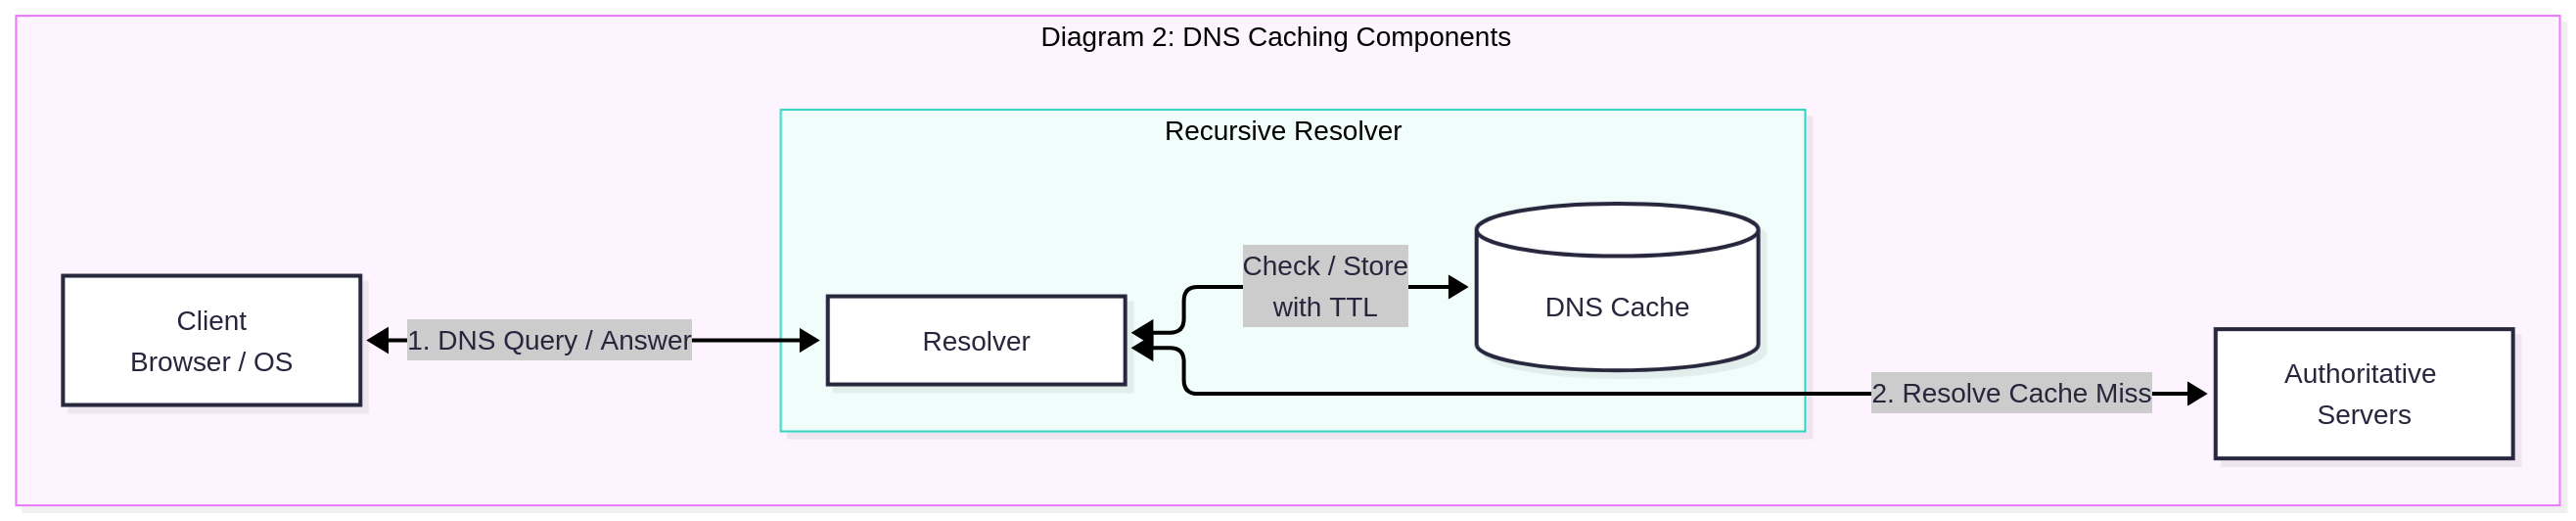
\includegraphics[width= 1\textwidth]{figures/dns-caching}
	\caption[DNS caching]{
		DNS caching.
		Initially generated using Gemini 4 Argon with the prompt
		``Generate a high-level mermaid diagram illustrating DNS recursive resolver caching, with its components and interactions'' on 17.10.2026, modified by the author.
		
	}
	\label{fig-caching}
\end{figure}

\subsection{DNS Privacy: DoH \& ODoH}
\label{sec:dnsprivacy}

Traditionally, DNS messages have been transported without encryption, usually encapsulated over User Datagram Protocol (UDP) \citep{rfc1034}. This implies that network observers can read all the packet information, including Source IP Address and the requested domain name, potentially exposing browsing activity. Furthermore, the lack of encryption in traditional DNS increases its vulnerability to network attacks. An attacker may intercept a query and try to manipulate the response to redirect the victim to a malicious location \citep{rfc3833}.

\citet{rfc8484} solved the lack of encryption by transporting DNS over HTTPS, using Transport Layer Security (TLS) for encryption, integrity and confidentiality. This is done by encapsulating DNS messages in HTTP requests under HTTPS URIs, using either POST or GET methods. DoH prevents network observers and/or attackers from reading the DNS queries, partly protecting users' privacy. However, it still has a key limitation: the resolver has access to the unencrypted DNS message and can associate it with the client's IP address.

To solve this problem, \citet{singanamalla2020oblivious} introduced \textit{Oblivious DNS over HTTPS (ODoH)}, which introduces a proxy between the client and the resolver. The client encrypts the DNS message for the resolver, so the proxy does not have access to the contents of the query, and forwards the encrypted DNS message, as illustrated in Figure~\ref{fig-odoh}. Assuming the proxy and the resolver do not collude, the client's IP address is unknown for the resolver, and the queried domain name is unknown for the proxy, so the users' privacy remains protected. However, this introduces a new problem: encryption makes two equal DNS queries different to the proxy, so conventional caching becomes impossible \citep{niroula2026codoh}.

\begin{figure}[H]
	\centering
	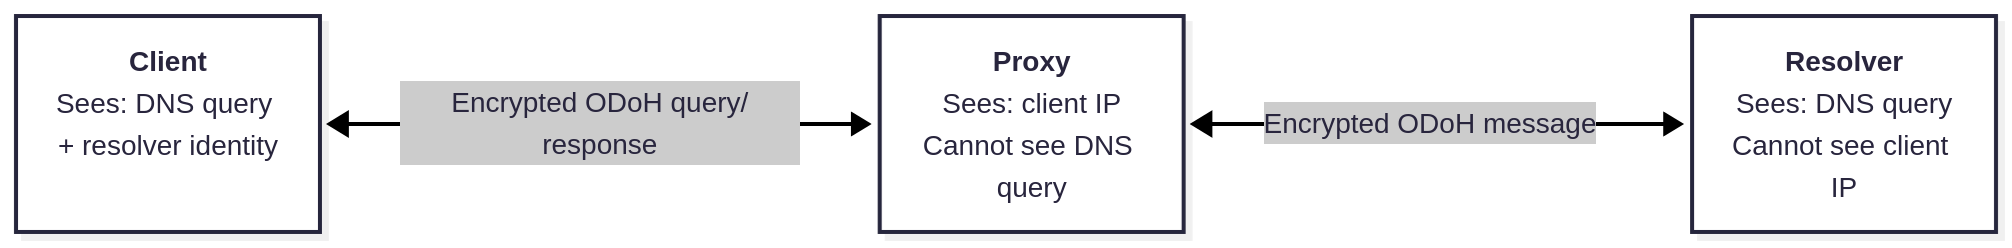
\includegraphics[width= 1\textwidth]{figures/oblivious-doh}
	\caption[ODoH Architecture]{
		ODoH Architecture.
		Generated using GPT 5.6 Sol High with the prompt
		``Create a simple mermaid LR diagram to illustrate ODoH: Client <-> Proxy <-> Resolver. Show what's visible to each party'' on 17.10.2026
		
	}
	\label{fig-odoh}
\end{figure}

\subsection{Trusted Execution Environments (TEEs) \& Remote Attestation}
\label{sec:tees}

Although encryption protects sensitive information in transit and rest, processing this information usually requires it to be decrypted and loaded into memory. Traditionally, privileged software such as the Operating System has been allowed to access and manipulate all computer memory. Consequently, applications must trust the environment in which they execute. \textit{Trusted Execution Environments (TEEs)} address this limitation by providing hardware-enforced isolation. \citep{7345265}

\textit{Intel SGX} \citep{cryptoeprint:2016/086} is a TEE that extends the Intel architecture to guarantee isolated execution in protected containers called \textit{enclaves}, and permits proving to a remote computer that it is communicating with a specific secure container using \textit{software attestation}. The proof is an attestation signature covering the container's initial state, a challenge random number produced by the remote computer, and a message produced by the container. This allows remote hosts to execute programs in a secure container, as illustrated in Figure~\ref{fig-sgx-secure}.

\begin{figure}[H]
	\centering
	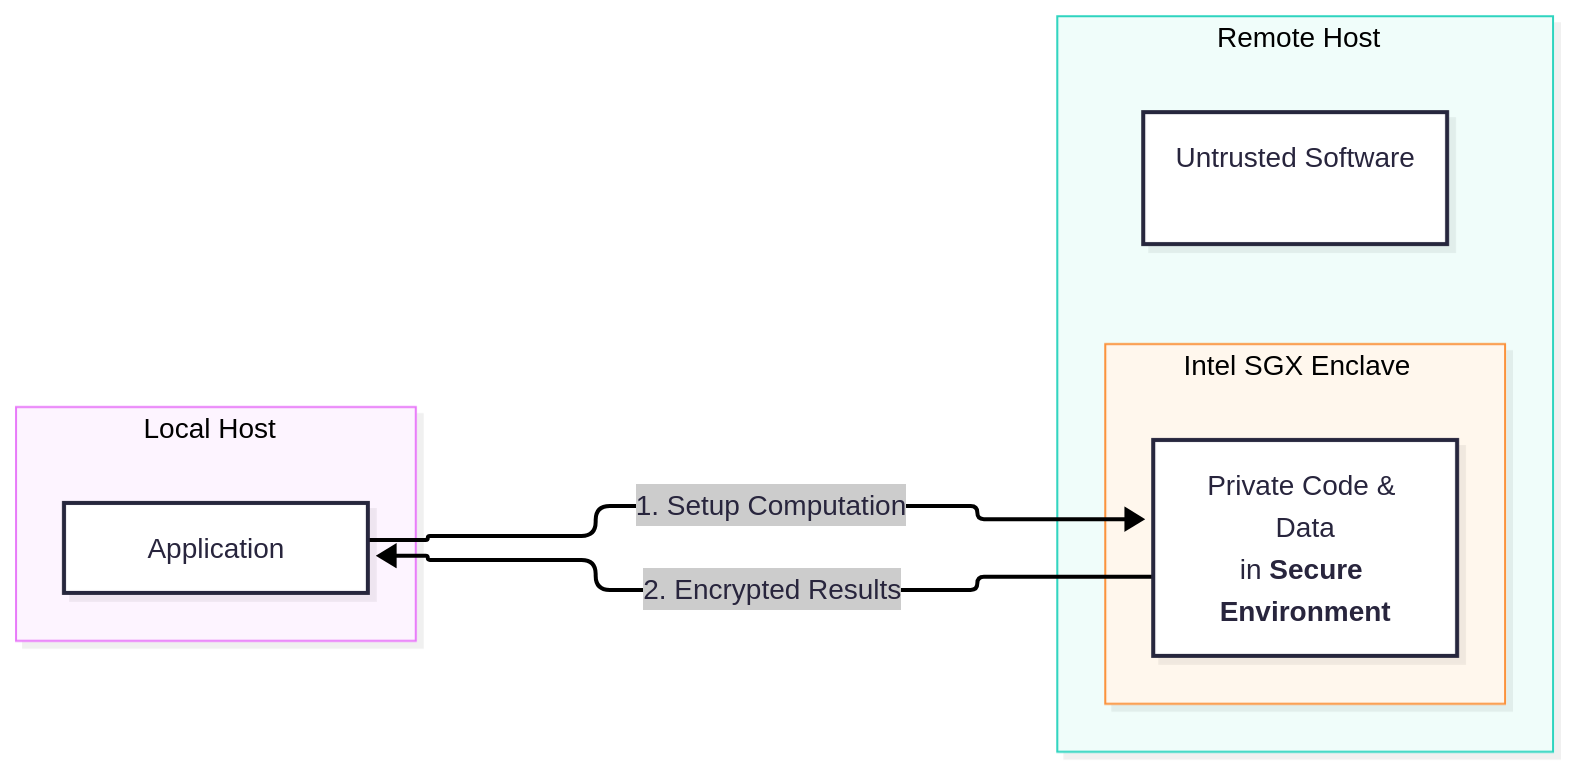
\includegraphics[width= 0.7\textwidth]{figures/intel-sgx-remote}
	\caption[Intel SGX Secure Remote Computation]{
	Intel SGX Secure Remote Computation. A local host setups computation in a remote secure container (enclave), and receives encrypted results from that computation.
	}
	\label{fig-sgx-secure}
\end{figure}

\subsection{Oblivious RAM (ORAM)}
\label{sec:oram}

Even though Intel SGX's enclaves have their memory encrypted \citep{cryptoeprint:2016/086}, this alone may not be enough to protect their data. An attacker observing memory access patterns may be able to infer sensitive information, even if the underlying information is encrypted. \citet{oramgoldreich} introduced \textit{Oblivious RAM (ORAM)} to address this problem by transforming how memory is accessed, preventing observable access patterns from revealing what data is being accessed.

\textit{Path ORAM} \citep{pathoram} is a modern ORAM protocol that organizes encrypted data blocks by assigning them to leafs in a binary tree. After each access, the block is moved to a different leaf, preventing repeated access to the same data block from revealing access patterns. However, this introduces significant memory access overhead when compared to traditional memory access.

\subsection{Related work}
\label{sec:relatedwork}

% TODO

Here, you include short descriptions of similar work and explain \textit{how} they are different from the main content you have presented.

Level of detail similar to an abstract.

\section{CODoH Design}
\label{sec:main}

\subsection{Design Goals}
\label{sec:designgoals}

ODoH separates the knowledge between two parties: the proxy, aware of the user's IP address, and the target, with access to the unencrypted DNS query  \citep{singanamalla2020oblivious}. However, effective conventional DoH proxy caching requires the proxy to be able to identify repeated requests \citep{rfc8484}, which is not possible with CODoH's encryption. CODoH's fundamental goal therefore is to implement a cache at the proxy while preserving ODoH's privacy enhancements \citep{niroula2026codoh}, in order to achieve \textit{performance requirements} and \textit{cache-specific security goals}.

\textbf{Performance requirements.} CODoH should reduce latency for cache hits relative to ODoH baseline; for cache misses, latency should not significantly differ relative to ODoH baseline. \citep{niroula2026codoh}

\textbf{Cache-specific attack vectors.} Caching introduces new attack vectors \citep{niroula2026codoh}. For example, in a \textit{set-difference (bracketing) attack}, a malicious proxy may:

(1) Learn the current cache state.

(2) Allow a victim query to proceed, queueing other traffic.

(3) Learn the cache state again.

(4) Compute the difference to isolate the newly added entry, potentially identifying the victim's query.

\textbf{Cache-specific security goals.} Given the new attack vectors,  CODoH aims to achieve the security goals below:

(G1) \textit{Authorized and fresh cached answer}. A proxy must not be able to cause clients to accept answers not authorized by the target, or answers with an expired TTL.

(G2) \textit{Cache-state indistinguishability}. The proxy must not be able to learn meaningful information about particular queries by comparing cache states across time, like in the previous example of a set-difference attack.

(G3) \textit{Query equality and profiling resistance}. The proxy must not be able to determine whether two DNS queries are equal by comparing them.

\subsection{Design Overview}
\label{sec:designoverview}

CODoH \citep{niroula2026codoh} aims to achieve its goals by following an architecture, illustrated in Figure~\ref{fig-codoh-arch}, with three independent parties: the \textit{client}, the \textit{proxy}, which contains the \textit{enclave}, and the \textit{DNS resolver}

\textbf{The client} is expected to have access to the HPKE public keys of the enclave and the target. Using these, it encrypts the query for both the enclave (CODoH query) and the target (ODoH query), and sends both encrypted queries to the proxy. Finally, it receives both encrypted DNS responses from the proxy, and decrypts them.

\textbf{The proxy} forwards both encrypted messages to the enclave and the target. In addition, it forwards encrypted responses from the enclave and the target, whose contents are encrypted, so whether it is a cache hit or miss is unknown to the proxy, and the client always needs to receive both responses.

\textbf{The enclave} contains the cache table, accessed using Path ORAM to avoid access patterns leaking information. Cache gets filled with signed and encrypted response batches received from the target, which include a trusted timestamp that ensures safe cache expiration and replay protection.

\textbf{The target} decrypts the DNS query and answers with an encrypted response whose private key is only known by the client. It has no way to identify the client, so privacy is preserved.

\begin{figure}[H]
	\centering
	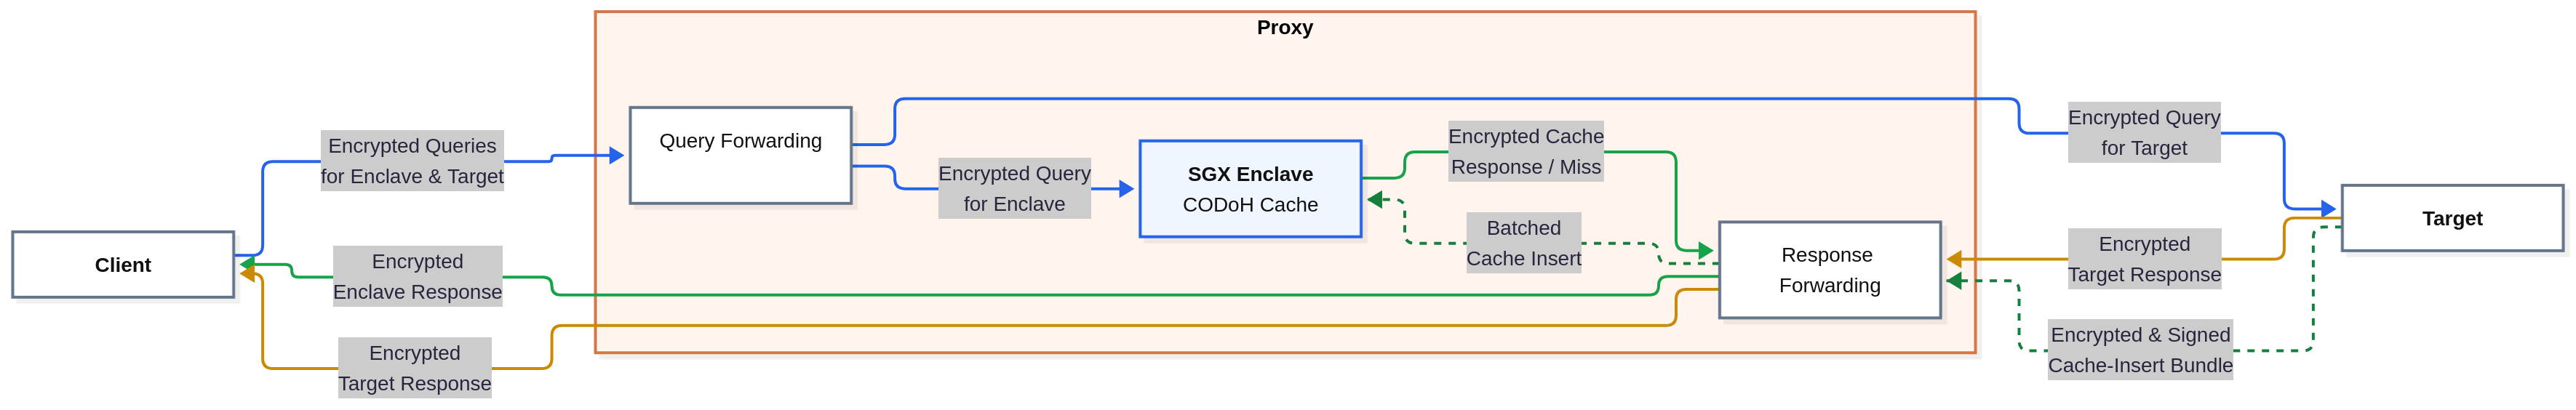
\includegraphics[width= 1\textwidth]{figures/codoh-arch}
	\caption[Simplified CODoH Architecture]{
		Simplified CODoH Architecture, adapted from \citet{niroula2026codoh}. The proxy forwards independently encrypted queries to the SGX enclave and target. The enclave provides privacy-preserving cache. Target provides signed and encrypted cache insert bundles with a trusted timestamp. Solid arrows represent queries and responses, while dashed arrows represent cache inserts. Blue arrows represent queries, red arrows represent cached responses and cache inserts, and yellow arrows represent target responses.
	}
	\label{fig-codoh-arch}
\end{figure}

\subsection{Security}
\label{sec:security}

As explained in Section~\ref{sec:designgoals}, caching introduces new attack vectors that may reveal or allow to infer sensitive information. This subsection examines the design decisions taken on CODoH \citep{niroula2026codoh} to protect from these.

\subsubsection{Cache State}
Sending encrypted requests to both the proxy and the target even on cache hits may look redundant. However, it is essential to prevent the proxy from being aware of whether a query was already cached, which, could reveal information to a malicious proxy. For example, the proxy may populate an empty cache with certain domains, and not let any new responses be inserted into the cache. In such case, any cache hit from a victim would certainly be a query to these domains.

\citet{niroula2026codoh} addressed this issue in CODoH by sending both encrypted requests to the enclave and the target in every request, even if it is a cache hit. In addition, to prevent cache hits from being distinguished from cache misses, the target resolver's response is always sent to the client, and cache messages contain padding. Padding prevents, for example, a cache miss being identified due to a smaller size.

\subsubsection{Set-Difference Attacks}
An attacker controlling the proxy may compare the states before and after a victim's query to detect what domains were queried. In order to mitigate it, the target resolver generates \textit{cover responses} and inserts them in the cache with real responses. However, if these are generated uniformly from a list of popular domains, an attacker could easily detect rare domains. Therefore, a realistic distribution from a realistic list of domains is necessary \citep{niroula2026codoh}.

Even then, each query produces only small updates, so the probability of the attacker simply guessing the victim's queried domain is high, unless a very large number of cover responses are introduced into the cache per response, which would create a large DNS resolution, bandwidth and cache maintenance overhead. Therefore, CODoH introduces \textit{batching} \citep{niroula2026codoh}, so, instead of caching every independent response, the resolver waits for a number of responses, before inserting them into the cache, reducing the overhead required for the same protection. This comes with the limitation of potentially increased cache misses, especially with larger batches and lower variability of domain names.

\subsubsection{Replay Attacks}
Since SGX enclaves do not provide a trusted clock, enclave cache in CODoH determines whether a cache entry's TTL has expired by having the resolver include a timestamp with every cache insert. In order to prevent against unauthorized inserts, this timestamp is signed with every insert \citep{niroula2026codoh}. However, even with a signed timestamp, a malicious proxy could re-insert an old insertion batch and roll-back in time, causing potentially incorrect answers to be served. Therefore, in CODoH, enclave cache rejects cache insertions older than the last previous insertion, with a configurable tolerance to prevent benign network delays from blocking insertions \citep{niroula2026codoh}.

\subsubsection{Controlled Cache State}

A malicious proxy may try to control the cache state to facilitate set-difference attacks.

\textbf{Enclave Restarts}. For example, the proxy could restart the enclave to have an initial empty state, and then comparing it with the next state would be much simpler. CODoH \citep{niroula2026codoh} enables accountability by generating new key pairs on each restart, facilitating detection. However, since that alone does not prevent the attacks, the enclave has a \textit{defensive mode} that returns cache misses for every request, removing the ability to check the cache state. The enclave starts in defensive mode as a warm-up on every restart, not serving cache hits until certain configurable threshold has been reached.

\textbf{Cache Omission}. With the same purpose, the proxy may also skip certain resolver responses from being inserted into the cache. For example, it may check for a domain in the cache after every request to check whether that client queried the domain. In such case, the proxy would want to prevent the cache to be populated from that response, as otherwise future clients could not be distinguished from the probe query's cached entry.

This attack gets mitigated in CODoH \citep{niroula2026codoh} by having the enclave track what queries it has not received a matching resolver cache insert for. When the count of queries without matching cache insert reaches a threshold, the enclave enters the same defensive mode introduced previously, disabling cache hits temporarily.

\subsubsection{Memory Access Patterns}

Intel SGX encrypts memory \citep{cryptoeprint:2016/086}. However, if the proxy runs on an untrusted machine, where some attacker can see what memory addresses are accessed by the enclave, it could infer whether two clients are querying the same domain checking if memory access patterns match, or simulate its own queries and compare their memory access patterns with a client's query ones, potentially fingerprinting cache entries and revealing the queried domains.

CODoH \citep{niroula2026codoh} addresses this by using ORAM, which makes memory access patterns indistinguishable. Two consecutive lookups to the same cache entry will not share memory access patterns, and therefore malicious actors can not infer what domain a user enters. In addition, the enclave performs a fixed number of ORAM operations per lookup or insert, reducing timing variation that could also reveal information from patterns in time to access entries.

\section{Performance}

\citet{niroula2026codoh} evaluated CODoH's performance on an implementation as a set of plugins for CoreDNS, a DNS server written in Go \citep{belamaric2019learning} that facilitates controlled comparisons by using a plugin for each protocol variant (DoH, ODoH and CODoH). This section examines the methodology and results of performance aspects from \citet{niroula2026codoh}'s CODoH evaluation.

\subsection{End-to-End Benchmarks}

\subsubsection{Methodology}

\textbf{Experimental setup}. \citet{niroula2026codoh} deployed the system across three Azure VMs in separate regions to capture realistic network latencies. The \textit{client} was deployed on a Standard D2alds v6 (2 vCPUs, 4 GiB), the \textit{proxy} on a Standard DC4s v2 (4 vCPUs, 16 GiB,
112 MiB EPC) with Intel SGX support, and the \textit{target} on a standard D2s v3 (2 vCPUs, 8 GiB), using Ubuntu 24.04 LTS, Go 1.25 and EGo 1.8.1

The target VM's CoreDNS instance uses a local Unbound recursive resolver in the same VM \citep{niroula2026codoh}, mitigating potential latency that could appear if it were external. Caching is enabled in its default setting, but flushed between workloads to ensure independent measurements \citep{niroula2026codoh}. However, the usage of a recursive resolver that queries external servers implies that the normal variation of network conditions may cause variability in the results unrelated to the configuration, especially in workloads with less cache hits at the resolver level.

\textbf{Configurations}. \citet{niroula2026codoh} used five configurations for the experiments: C1 (traditional DNS over HTTPS), C2 (Oblivious DNS over HTTPS), C3 (Cached ODoH on SGX without CODoH's defense mechanisms from Section~\ref{sec:security}), C4 (CODoH, running in normal userspace instead of an Intel SGX enclave) and C5 (Full CODoH)

\textbf{Workloads} \citet{niroula2026codoh} used three different workloads: \textit{Cold}, with 10,000 unique domains queried, so every query is a cache miss; \textit{Zipf}, with 10,000 queries drawn from an Zipf distribution over 1,000 domains, trying to simulate real traffic; And \textit{warm}, with 10,000 queries for a single domain, so almost every query is a cache hit.

These workloads were used aiming to understand whether CODoH has fulfilled its latency goals, examined on Section~\ref{sec:designgoals}, with Cold aiming to show its impact on cache misses latency, zipf on real traffic, and warm on cache hits. 

\subsubsection{End-to-end latency}

In \citep{niroula2026codoh}'s experiments, CODoH substantially improved ODoH's latency for both zipf (48.59ms/22.34ms) and warm (47.97ms/17.96ms) workloads, as illustrated in Figure~\ref{fig-odoh-latency}. Cold workload shows a small difference (108.49ms/97.20ms) that may be caused by the variability in upstream DNS resolution latency.

\begin{figure}[H]
	\centering
	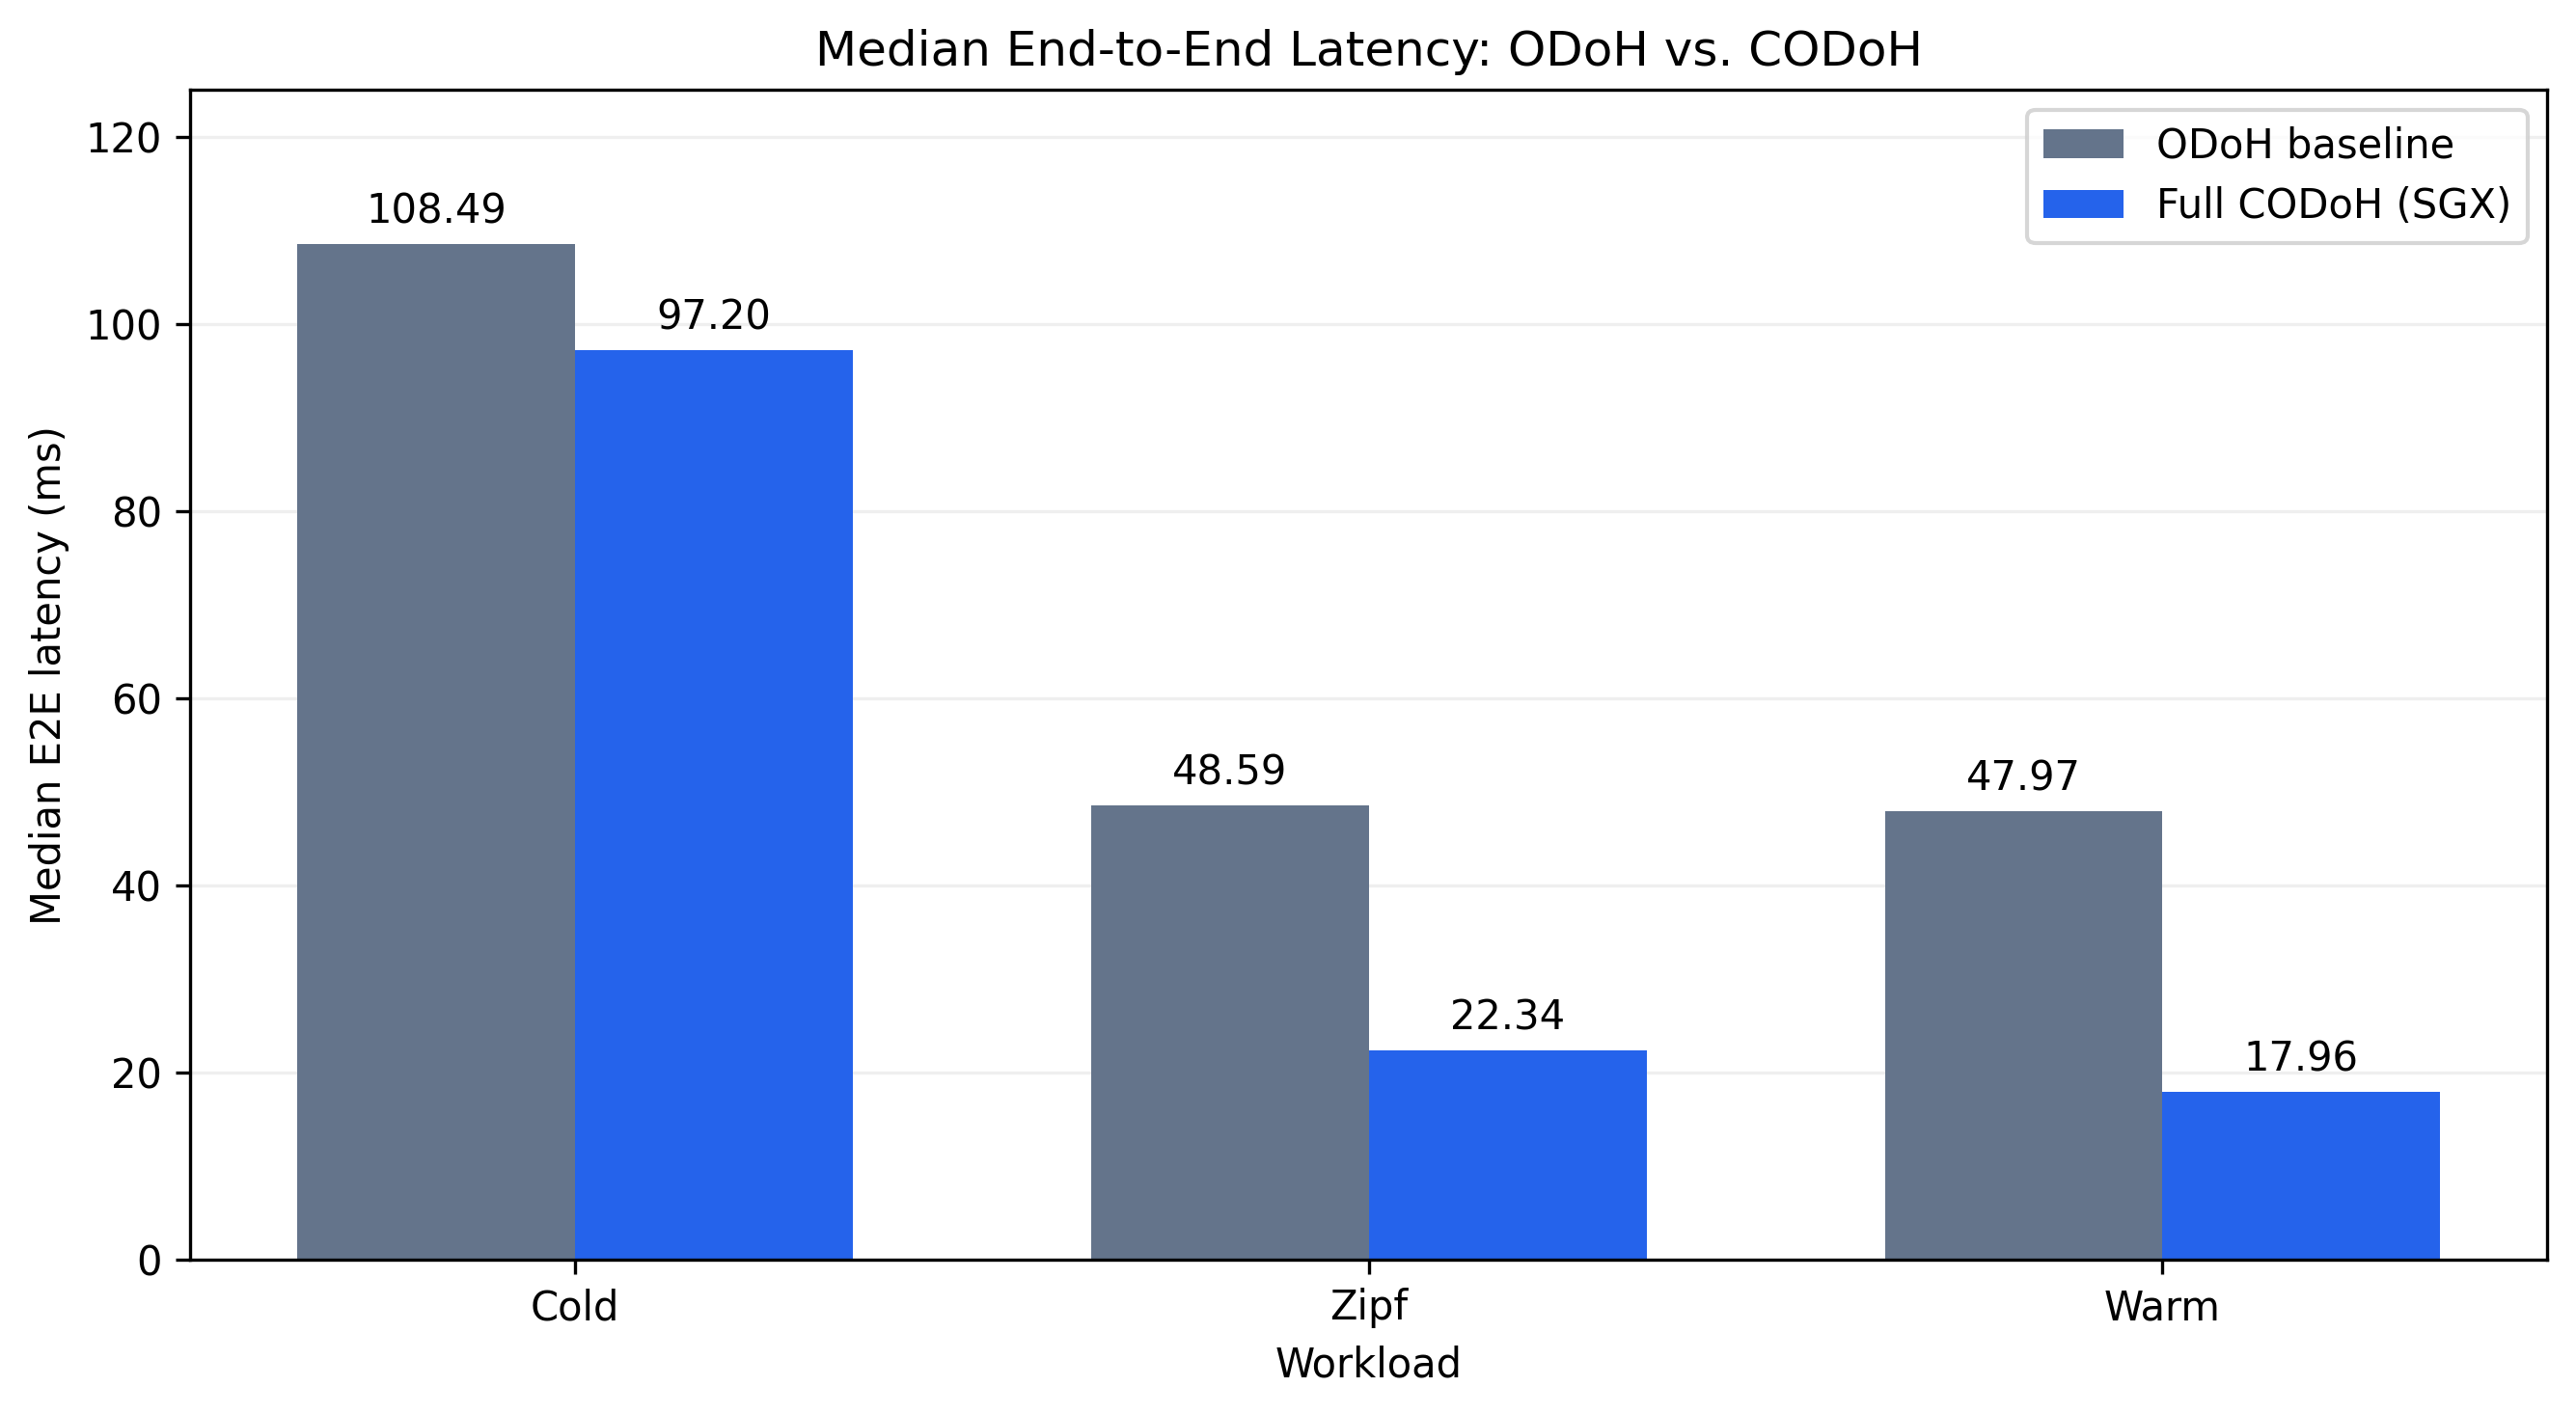
\includegraphics[width= 0.8\textwidth]{figures/codoh-latency}
	\caption[CODoH Latency]{
		CODoH Median Latency (ms) comparison between ODoH Baseline and Full CODoH. Adapted from Table 3 \citep{niroula2026codoh}
	}
	\label{fig-odoh-latency}
\end{figure}


\section{Conclusion}
\label{sec:conclusion}

\section{Use of generative digital tools}

Large Language Models (LLMs), specifically Gemini and ChatGPT models, have been used in the creation of this report for the following purposes:

A. Research and understanding concepts, using prompts of the type: "How does [...] work?", "Explain [...]", "What solutions similar to [...] have been used to solve [...] problem?", "What is [...]?", "What problem does [...] solve?"

B. Generation of diagrams. All prompts were of the type: "Generate a mermaid diagram illustrating [...]"

C. Concept checking. Prompts of the type: "Is [...] conceptually correct?", "Is [...] correctly expressed?"


\bibliographystyle{apalike}

\bibliography{references}


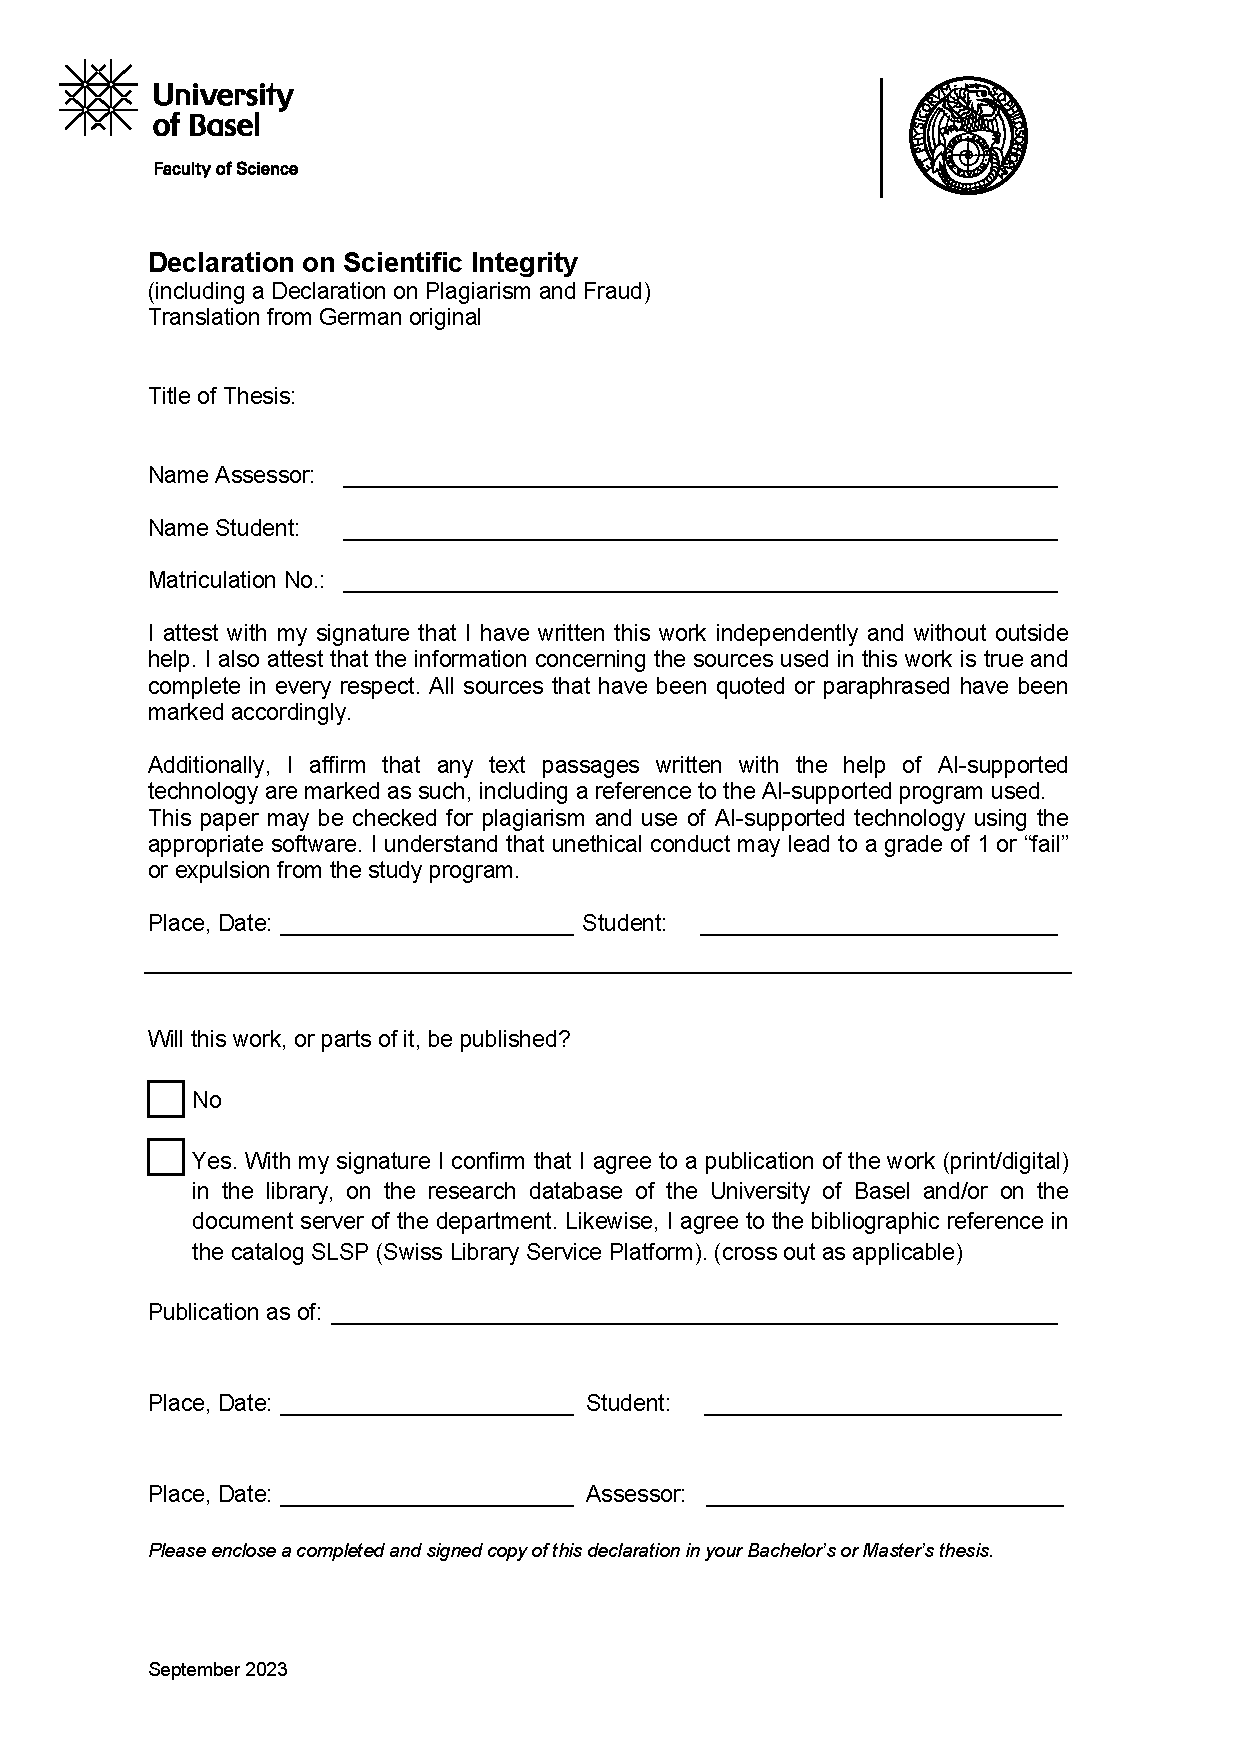
\includegraphics[width=\textwidth]{wissensch_Redlichkeit_E_09-2023}


\end{document}
